\chapter{Simulation and Results}
\label{chap4}
In the previous chapter, we have discussed about our methodology for this project while giving details about block diagram, system model, flow chart, software selection of this project. In this chapter, we will provide source code, and simulation and results of the project.
\section{Simulation Results}
As discussed in the previous chapter in the section of software selection, we have used MATLAB to simulate our project.
We have used two MATLAB function. In the first file, we have used that for the recording of the input signal where as the second file is accessing the input signal while calling that audio signal file and is performing the rest of the operation on that. Each line is properly comment to understand the use of that command.\\
{ \small \bfseries Note: Make sure both file should be in the same folder.}
\section{Source Code}
  \begin{lstlisting}[frame=single]
    % First(1) File
clc %Clear command window.
close all %closes all the open figure windows.

% sampling frequency
F = 32000;

%  recording speech on MATLAB
%  5*F is recording speech of 5 secs of sampling frequency
%  datatype to store the sound

y  = wavrecord(5*F, F, 'int16');
%Record sound using Windows audio input device.
%Y = wavrecord(N,FS,CH) records N audio samples at FS Hertz from
%CH number of input channels from the Windows WAVE audio device.
%playing recorded speech

wavplay(y, F);
% wavplay Play sound using Windows audio output device.
%wavplay(Y,FS) sends the signal in vector Y with sample frequency
%of FS Hertz to the Windows WAVE audio device.

audiowrite('project.wav',y, F)
%it will write the speech signal of the current file(save in memory)
%audiowrite write audio files
%audiowrite(FILENAME,Y,FS)  writes data Y to an audio
%file specified by the file name FILENAME, with a sample rate
%of FS Hz.
  \end{lstlisting}
  
\begin{lstlisting}[frame=single]
    % Second(2) File
clc
% (part a)
% wavread will read the .wav file in which speech is recorded
% y is samples or the input signal
% fs is the sampling frequency
[y,fs] = wavread('project.wav');
wavplay(y,fs);   %wavplay Play sound using Windows audio output device.
subplot(2,1,1)
% plotting frequency spectrum
% y is input signal
%freqz Frequency response of digital filter
freqz(abs(y))
% setting axis limits
x = linspace(0,0.1);    %linspace Linearly spaced vector.
xlim([0 0.1])   % xlim X limits.
ylim([-80 80])  % ylim Y limits.
title('Freq doamin magnitude spectrum of speech.');
subplot(2,1,2)% subplot Create axes in tiled positions.
% plotting time spectrum
plot(y),grid on;            % Linear plot &  Grid lines.
title('Time domain');       %Graph title.
xlabel('Seconds');         %X-axis label.
ylabel('Apmlitude');        %ylabel

% figure used to make the graphs appear in different windows
figure;
% fft is Fourier Transform to find highest frequency of signal
z=fft(y);
plot(abs(z)),grid on;           % Linear plot &  Grid lines.
title('Highest frequency');     %graph title
xlabel('Freq Hz');              %x-axis label
ylabel('Power');                %y-axis label

figure;
% (part b)
subplot(2,1,1)% subplot Create axes in tiled positions.
% decimating or downsampling the speech by facor 2
y1 = decimate(y,2)
%decimate is a low pass filter
freqz(abs(y1))%freqz frequency response of digital filter
x = linspace(0,0.1);    %linspace Linearly spaced vector.
xlim([0 0.1])           %x-axis limit
ylim([-80 80])          %y-axis limit
title('Freq doamin magnitude spectrum after decimating by 2');%graph title
subplot(2,1,2)% subplot Create axes in tiled positions.
plot(y1),grid on;% Linear plot &  Grid lines.
title('Time domain');       %graph title
xlabel('Seconds');          %x-axis label
ylabel('Apmlitude');        %y-axis label
wavplay(y1,fs);   %wavplay Play sound using Windows audio output device.


figure;         % figure Create figure window.
% (part c)
subplot(2,1,1)
% decimating by 4
y2 = decimate(y,2*2)
%decimate Resample data at a lower rate after lowpass filtering.
freqz(abs(y2))%freqz frequency response of digital filter.
x = linspace(0,0.1); %linearly spaced vector.
xlim([0 0.1]) %x-axis limit
ylim([-80 80])%y-axis limit
title('Freq Doamin Magnitude Spectrum After Decimating by 4');%graph title
subplot(2,1,2)% subplot Create axes in tiled positions.
plot(y2),grid on;% Linear plot &  Grid lines.
title('Time domain'); %graph title
xlabel('Seconds'); %x-axis label
ylabel('Apmlitude');%y-axis label
wavplay(y2,fs); %wavplay play sound using windows audio output device.


figure; %create figure window
% (part d)
subplot(2,1,1)% subplot Create axes in tiled positions.
% decimating by 8
y3 = decimate(y,2*2*2)
%decimate resample data at a lower rate after lowpass filtering
freqz(abs(y3)) %frequency response of digital filter.
x = linspace(0,0.1); %linearly spaced vector
xlim([0 0.1]) %x-axis limit
ylim([-60 60])%y-axis limit
title('Freq doamin magnitude spectrum after decimating by 8');%graph title
subplot(2,1,2)% subplot Create axes in tiled positions.
plot(y3),grid on;% Linear plot &  Grid lines.
title('Time domain'); %graph title
xlabel('Seconds');%x-axis label
ylabel('Apmlitude');%y-axis label
wavplay(y3,fs); %plays sound using windows audio output device


figure;%create figure window
% (part e)
subplot(2,1,1)% subplot Create axes in tiled positions.
% decimating by 16
% decimate resample data at a lower rate after lowpass filtering
y4 = decimate(y,2*2*2*2)
freqz(abs(y4))%frequency response of digital filter.
x = linspace(0,0.1);%linearly spaced vector
xlim([0 0.1])%x-axis limit
ylim([-50 50])%y-axis limit
title('Freq doamin magnitude spectrum after decimating by 16');%graph title
subplot(2,1,2)% subplot Create axes in tiled positions.
plot(y4),grid on;% Linear plot &  Grid lines.
title('Time domain');%graph title
xlabel('Seconds');%x-axis label
ylabel('Apmlitude');%y-axis label
wavplay(y4,fs);%plays sound using windows audio output device

z=fft(y4);
figure;
plot(abs(z)),grid on;
\end{lstlisting}
\clearpage
\section{Statistical Analysis}
\label{analysis}
Frequency spectrum of Input signal and  input signal in time domain is Fig. \ref{result1} .
\begin{figure}[H]  %h=positioning
\begin{center}
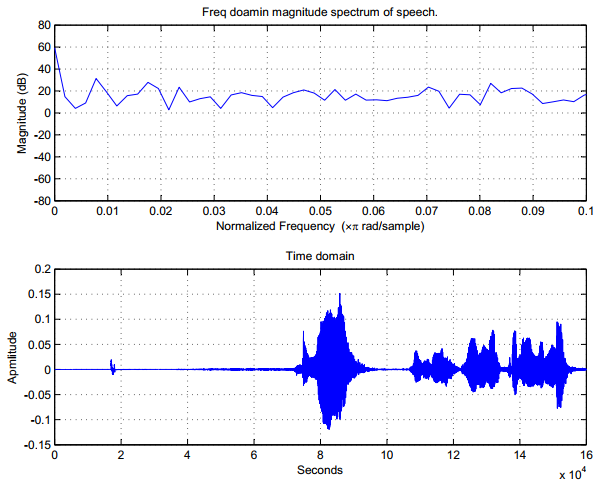
\includegraphics[scale=0.80]{Chapter4/result1}
\caption{Comparison of Frequency Spectrum and Time Domain Graph of Input Signal }
\label{result1}
\end{center}
\end{figure}

The highest frequency of recorded speech signal is 327kHz from fft is Fourier Transform to find highest frequency of signal which is shown in Fig. \ref{result2}

\begin{figure}[H]  %h=positioning
\begin{center}
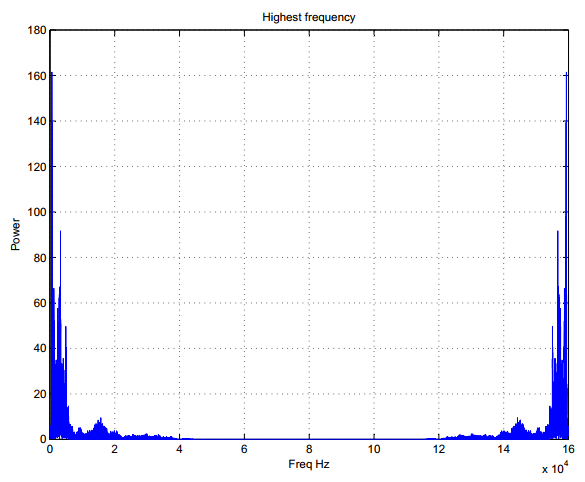
\includegraphics[scale=0.65]{Chapter4/result2}
\caption{Fourier Transform of the Input Signal }
\label{result2}
\end{center}
\end{figure}
Data transmitted per unit time is increased so does the speed of transmission or the speed
of speech is increased. Another thing we observed by decimating by 2 is that the
amplitude of frequency magnitude spectrum is got lowered from amplitude of original
frequency magnitude spectrum.\\\\
 
For example, if we take any sample point let�s say at 0.1,
the amplitude of original frequency magnitude spectrum at that sample point is almost
30dB but when decimated by 2 the amplitude of decimated frequency magnitude
spectrum goes to 28dB. Therefore, speech is not that much clear to understand than
original speech and time is reduced as shown in the Fig. \ref{result3}.

\begin{figure}[H]  %h=positioning
\begin{center}
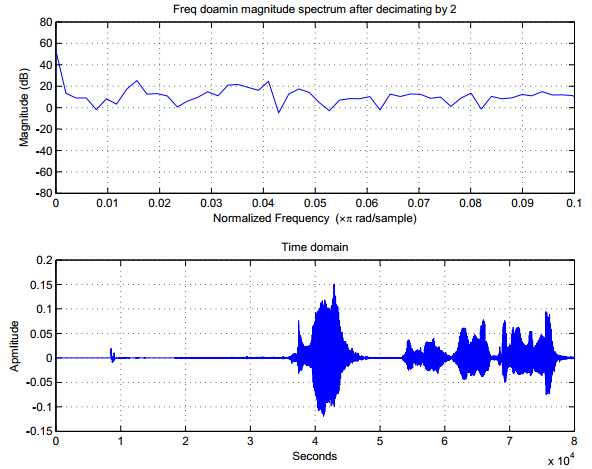
\includegraphics[scale=0.90]{Chapter4/result3}
\caption{Comparison of Frequency Spectrum and Time Domain Graph of Input Signal After Decimating by 2 }
\label{result3}
\end{center}
\end{figure}
Data transmitted rate is much more increased. By decimating by 4 the amplitude of
frequency magnitude spectrum is got much lowered from amplitude of original frequency
magnitude spectrum.\\\\
 For example, if we take any sample point let�s say at 0.1, the amplitude of original frequency magnitude spectrum at that sample point is almost 30dB but when decimated by 4 the amplitude of decimated frequency magnitude spectrum goes
to 25dB. The decimated speech is very rough and not clear enough to understand because
time is more decreased as shown in the Fig. \ref{result4}.

\begin{figure}[H]  %h=positioning
\begin{center}
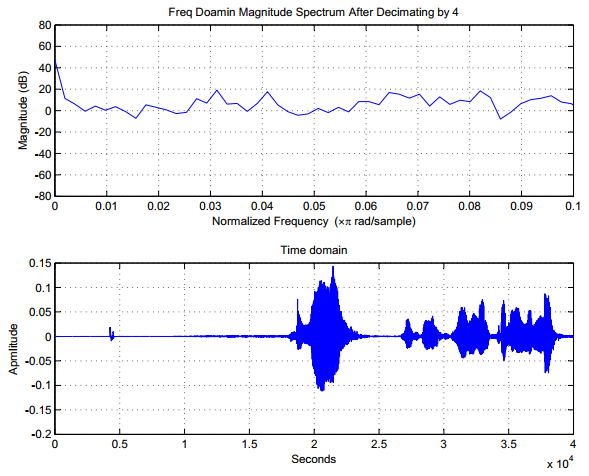
\includegraphics[scale=0.90]{Chapter4/result4}
\caption{Comparison of Frequency Spectrum and Time Domain Graph of Input Signal After Decimating by 4 }
\label{result4}
\end{center}
\end{figure}


Decimation reduces the original sample rate of a sequence to a lower rate. It is the opposite of interpolation. decimate lowpass filters the input to guard against aliasing and downsamples the result. When using the FIR filter, decimate filters the input sequence in only one direction. This conserves memory and is useful for working with long sequences. In the IIR case, decimate applies the filter in the forward and reverse directions using filtfilt to remove phase distortion. In effect, this process doubles the filter order. In both cases, the function minimizes transient effects at both ends of the signal by matching endpoint conditions\\\\
Data transmitted per unit time is much more increased and the speed of transmission or
the speed of speech is increased. Another thing we observed by decimating by 8 is that
the amplitude of frequency magnitude spectrum is got lowered from amplitude of original
frequency magnitude spectrum.\\\\
For example, if we take any sample point lets say at 0.1,
the amplitude of original frequency magnitude spectrum at that sample point is almost
30dB but when decimated by 8 the amplitude of decimated frequency magnitude
spectrum goes to 18dB. The speech is played so fast that the speech is almost impossible
to understand, time is much more reduced as shown in the Fig.\ref{result5}.

\begin{figure}[H]  %h=positioning
\begin{center}
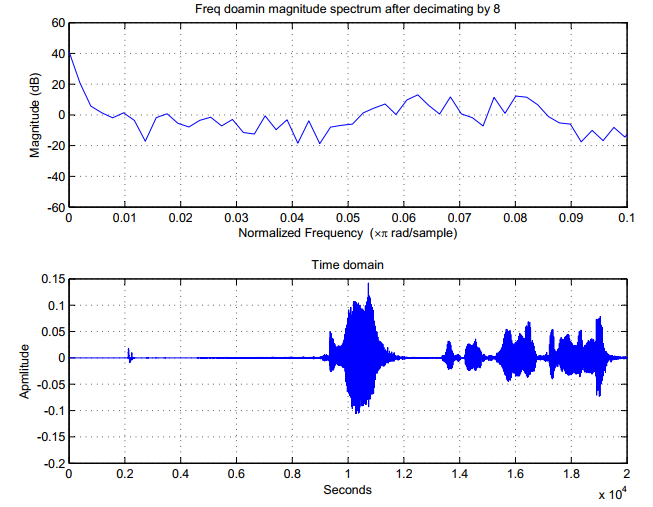
\includegraphics[scale=0.90]{Chapter4/result5}
\caption{Comparison of Frequency Spectrum and Time Domain Graph of Input Signal After Decimating by 8}
\label{result5}
\end{center}
\end{figure}

decimate creates a lowpass filter. The default is a Chebyshev Type I filter designed using cheby1. This filter has a normalized cutoff frequency of 0.8/r and a passband ripple of 0.05 dB. Sometimes, the specified filter order produces passband distortion due to round-off errors accumulated from the convolutions needed to create the transfer function. decimate automatically reduces the filter order when distortion causes the magnitude response at the cutoff frequency to differ from the ripple by more than $1/10^6$.\\
When the 'fir' option is chosen, decimate uses fir1 to design a lowpass FIR filter with cutoff frequency $1/r$.\\\\
Data transmitted per unit time is so much increased Another thing we observed by
decimating by 16 is that the amplitude of frequency magnitude spectrum is got lowered
from amplitude of original frequency magnitude spectrum.\\\\
For example, if we take any sample point let�s say at 0.1, the amplitude of original frequency magnitude spectrum at
that sample point is almost 30dB but when decimated by 16 the amplitude of decimated
frequency magnitude spectrum almost goes to 1dB. The rate of speech is so less that the
speech is impossible to understand, time is much more reduced as shown in the Fig. \ref{result6}.

\begin{figure}[H]  %h=positioning
\begin{center}
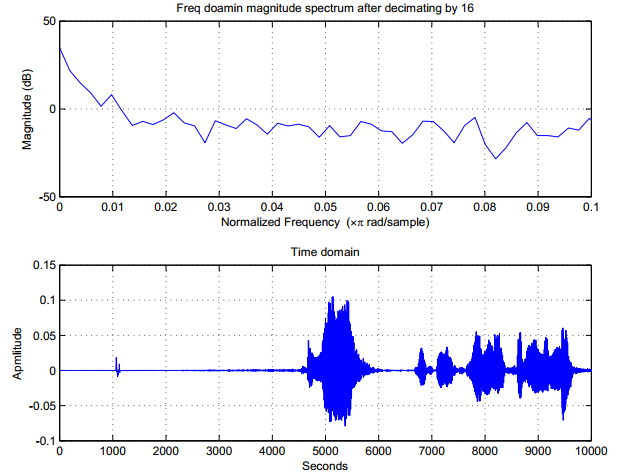
\includegraphics[scale=0.90]{Chapter4/result6}
\caption{Comparison of Frequency Spectrum and Time Domain Graph of Input Signal After Decimating by 16}
\label{result6}
\end{center}
\end{figure}